\documentclass[jair,twoside,11pt,theapa]{article}
\usepackage{jair, theapa, rawfonts}
\usepackage{graphicx}

\jairheading{?}{YYYY}{1-??}{M/YY}{M/YY}
\ShortHeadings{Standard Machine Learning Language (SML)}
{Ikegwu, Hao, \& Brunner}
\firstpageno{25}

\begin{document}

\title{Standard Machine Learning Language}

\author{\name Kelechi Ikegwu \email ikegwu2@illinois.edu \\
       \addr 226 Astronomy Building, MC-??? \\1002 W. Green St.\\ Urbana, IL  61801
       \AND
       \name Micheal Hao  \email ???@illinois.edu \\
       \addr ???
       \AND
       \name Robert Brunner \email bigdog@illinois.edu\\
       \addr 226 Astronomy Building, MC-221 \\1002 W. Green St.\\ Urbana, IL  61801}

% For research notes, remove the comment character in the line below.
% \researchnote

\maketitle


\begin{abstract}
Standard Machine Learning Language (SML) is a language agnostic framework that integrates a query-like language to simplify the development for a variety of state-of-the-art machine learning pipelines. Emphasis was placed on ease of use and abstracting the complexities of machine learning from the end user encouraging it's use in professional and academic settings from a variety of disciplines. SML's architecture is discussed, followed by multiple interfaces that one could use to interact with SML. We then apply SML to a few research problems and compare the complexities for multiple problems. Lastly we perform a case study on SML. The source code and documentation for SML is open sourced and publicly available on github \cite{ginsberg}.
\end{abstract}

\section{Introduction}
\label{Introduction}

Machine Learning has simplified the process of solving a vast amount problems in a variety of fields by learning from data. In most cases machine learning has become more attractive than manually creating programs to solve these same issues. However they're a lot of nuisances (that a novice may be unfamilar with) involved when developing machine learning pipelines \cite{pedros:fewUsefulThings} and if they are not taken into consideration one may not receive satisfactory results. In addition to this, an experience user may not want to deal with [REASONS HERE]. In this paper we introduce Standard Machine Learning Language (SML)  which helps to combat these two use cases.


The overall objective of the SML is to provide a level of abstraction which simplifies the development process of machine learning pipelines. Consequently this enables researchers and industry professionals without a background in this area to use machine learning to solve problems. We developed a query like language to which serves as an abstraction from writing actual machine learning code see Figure \ref{fig:sml-ex-1} for an example.   

\begin{figure}
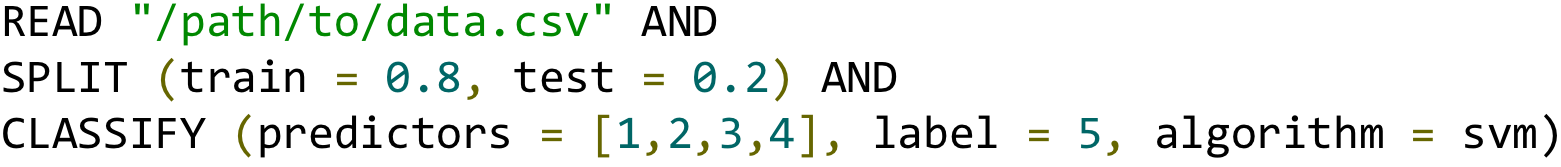
\includegraphics[width=0.6\textwidth]{figs/sml-ex-1.png}
\centering
\caption{Example of a SML Query. TODO: FIX COLOR SYNTAX}
\label{fig:sml-ex-1}
\end{figure}

\section{Related Works}
\label{RelatedWorks}

Related Works Stuff

\section{Grammar}
\label{grammar}

Grammar Stuff

\section{SML's Architecture}
\label{sml-architecture}

Architecture Stuff

\subsubsection{Model Phase}
model phase
\subsubsection{Apply Phase}
apply phase
\subsubsection{Metrics Phase}
It's often useful to visualize the data that one works with; it's also beneifical to see the performance metrics of your machine learning algorithm to better understand ones data. By default if you specify the `PLOT` keyword in a query, SML will execute the metrics phase. Figure \ref{fig:metric-phase} displays a block diagram of the metric phase of SML. SML performs a dictionary lookup with the average complexity of O(1) to find specific terms that are in the query. For the example in Figure \ref{fig:metric-phase} we specified `PLOT` which instructs SML to create visualizations, with the `READ` keyword SML will create a lattice plot containing Kernel Density Estimates. Given an algorithm type such as Classification SML generates plots such as ROC Curves and Validation and Learning Curves. For a comprehensive list for the type of plots that SML can generate visit  \cite{}.

\begin{figure}
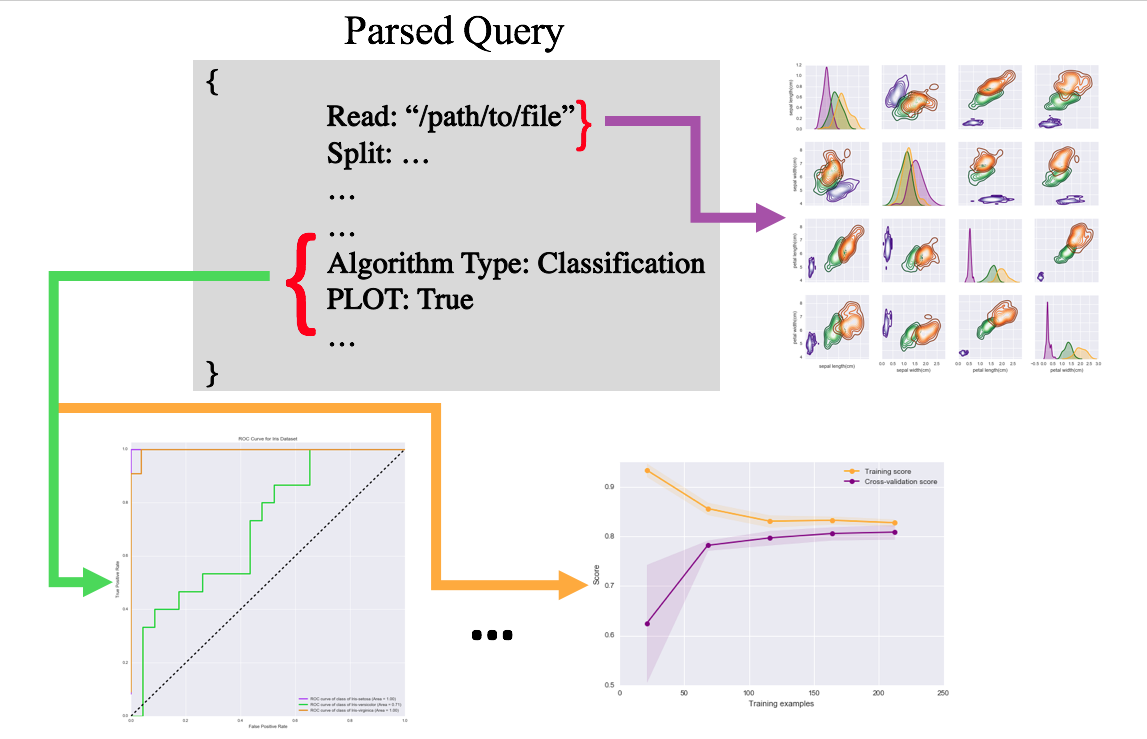
\includegraphics[width=0.6\textwidth]{figs/metric-phase.png}
\centering
\caption{Block Diagram of Metric Phase Architecture}
\label{fig:metric-phase}
\end{figure}

\subsubsection{Parser}
parser

\subsubsection{Connector}
connector

\section{Interface}
\label{interface}

They're multiple interfaces available for working with SML. We've developed a web tool that's publicly available which allows the user to interact with SML. There's also a REPL environment available that allows the user to interactively use SML. Lastly, users have the option to import SML into an existing pipeline to simplify the development process.

\section{Use Cases}
\label{use-cases}

use case stuff

\section{Case Study}
\label{case-study}
case study stuff

\section{Future Work}
\label{future-work}

future work stuff

\section{Conclusion}
\label{conclusion}
conclusion stuff

\acks{acknowledgments go here}

\appendix
\section*{Appendix X...}

Appendix goes here if needed.

\vskip 0.2in
\bibliography{main}
\bibliographystyle{theapa}

\end{document}






